% !TEX root = main.tex
\documentclass[conference]{IEEEtran}

% --- Packages ---
\usepackage{graphicx}
\usepackage{hyperref}
\usepackage{cite} 
\usepackage{amsmath} 
\usepackage{booktabs} 
\usepackage{algorithm}
\usepackage{algorithmic}
\renewcommand{\ttdefault}{txtt}

% --- Hyperlink Setup ---
\hypersetup{
    colorlinks=true,
    linkcolor=blue,
    urlcolor=cyan,
    citecolor=blue
}

% --- Title and Author ---
\title{Benchmarking Computational Pipelines for Conflict Data Analysis: Local Python vs. Cloud PostgreSQL vs. Distributed PySpark}
\author{
    \IEEEauthorblockN{Tain Yan Tun}
    \IEEEauthorblockA{
        \textit{Big Data Course} \\
        \textit{Asia Pacific International University} \\
        \textit{Department of Information Technology} \\
        Saraburi, Thailand \\
    }
}

\begin{document}

\maketitle

\begin{abstract}
    As the volume and complexity of event-based conflict datasets grow, researchers face critical architectural decisions regarding data processing pipelines. This study presents a comparative performance analysis of three distinct computational approaches: local in-memory processing using Python (Pandas), cloud-native relational querying via Supabase (PostgreSQL), and distributed big data processing using PySpark in a pseudo-distributed environment. Using the Myanmar Conflict Observatory dataset (n $\approx$ 100,000 events) as a case study, this research evaluates each approach across three dimensions: computational latency for Natural Language Processing (NLP) tasks, geospatial query throughput, and architectural scalability. The results demonstrate that while local Python remains optimal for rapid prototyping and medium-scale analysis, the cloud-native SQL approach offers superior concurrency for collaborative humanitarian monitoring, whereas PySpark provides the necessary horizontal scalability for global-scale conflict surveillance. This study provides a quantitative decision framework for choosing the optimal technology stack in conflict research and SDG monitoring.
\end{abstract}

\begin{IEEEkeywords}
    Analysis, PySpark, Supabase, PostgreSQL, Big Data, Myanmar Conflict, Performance Benchmarking.
\end{IEEEkeywords}

\section{Introduction}

The digitalization of conflict monitoring has transitioned from manual reporting to high-frequency, event-based data collection. Platforms such as the Armed Conflict Location \& Event Data Project (ACLED) now provide millions of georeferenced records, enabling granular spatiotemporal analysis of global hostilities \cite{raleigh2010introducing}. However, as datasets scale, traditional analytical workflows encounter bottlenecks in memory management and execution time.

Researchers in the humanitarian sector often operate within resource-constrained environments, making the choice of technology stack critical for both performance and cost-effectiveness. This study compares three prevalent architectural patterns:
\begin{itemize}
    \item \textbf{Local Python (Pandas):} The standard scientific computing stack, characterized by in-memory processing and ease of deployment.
    \item \textbf{Supabase (PostgreSQL):} A cloud-native, serverless PostgreSQL implementation that leverages SQL indexing and relational optimization.
    \item \textbf{PySpark (Hadoop):} A distributed computing framework designed for massive datasets that exceed the memory capacity of a single machine.
\end{itemize}

By benchmarking these technologies using the \textit{Myanmar Conflict Observatory} dataset, I aim to delineate the "performance crossover points" where one technology becomes significantly more advantageous than the others.

\section{Related Work}

The computational analysis of conflict has historically relied on static statistical models and manual data entry. However, the advent of "Big Data" and the formalization of data science as a predictive discipline \cite{dhar2013data} has necessitated more robust processing pipelines. 

\subsection{Evolution of Big Data Frameworks}
The introduction of MapReduce and the Hadoop Distributed File System (HDFS) revolutionized the ability to process unstructured data at scale \cite{white2012hadoop,dean2008mapreduce,ghemawat2003google}. While Hadoop provided a reliable foundation, its reliance on disk-based processing introduced high latency for iterative tasks. Spark emerged as a high-performance alternative, utilizing in-memory Resilient Distributed Datasets (RDDs) to achieve up to 100$\times$ faster processing for complex workflows \cite{zaharia2010spark}. In conflict research, Spark has been used primarily for large-scale social media sentiment analysis during civil unrest, but its application to event-level conflict logs remains an emerging field.

\subsection{Cloud-Native Databases in Research}
Simultaneously, the rise of "Backend-as-a-Service" (BaaS) platforms like Supabase has democratized access to enterprise-grade relational databases. By providing a managed PostgreSQL instance with built-in API layers and real-time capabilities \cite{supabase2024}, these platforms enable small research teams to deploy collaborative monitoring systems without the overhead of database administration. However, the performance trade-offs of using cloud-native SQL for analytical (OLAP) workloads versus traditional transactional (OLTP) tasks are not well-documented in the humanitarian context.

\subsection{Python in the Scientific Ecosystem}
Python has maintained its dominance in the scientific community through the "PyData" stack, primarily Pandas and NumPy \cite{mckinney2010data,vanderwalt2011numpy}. While highly efficient for exploratory data analysis (EDA), these tools are inherently limited by the physical RAM of the host machine, creating a scalability gap that this study seeks to quantify.

\section{Dataset and Case Study}

The comparison utilizes the Myanmar Conflict Observatory dataset, which synthesizes ACLED records from February 2021 to 2025. The dataset includes approximately 100,000 events, each containing spatial coordinates, actor taxonomies, and unstructured narrative notes. 

The following sections define two representative analytical tasks for benchmarking:
\begin{enumerate}
    \item \textbf{Task A: HICE Detection (NLP-heavy):} Extracting Health-Impacting Conflict Events (HICE) from unstructured text using a rule-based detection engine. This task is CPU-intensive and involves heavy string manipulation.
    \item \textbf{Task B: Geospatial Risk Matrix (IO-heavy):} Aggregating fatality and frequency metrics across 15 administrative regions to calculate a Severity Index. This task is IO-bound and involves group-by operations and geospatial joins.
\end{enumerate}

\section{Methodology}

\subsection{Architectural Implementation}
The three pipelines are implemented as follows:
\begin{itemize}
    \item \textbf{Python Pipeline:} Utilizes the \texttt{pandas} library for vectorised operations. Data is loaded from a local CSV file into memory. This represents the single-node, in-memory processing model.
    \item \textbf{Supabase Pipeline:} Data is hosted on a Supabase Pro instance (PostgreSQL 15). Queries are executed using standard SQL, leveraging B-tree indexes on \texttt{event\_date}, \texttt{region}, and \texttt{actor} columns. This represents the cloud-native relational model.
    \item \textbf{PySpark Pipeline:} Implemented using \textbf{PySpark 3.5 in Pseudo-Distributed Mode}. This configuration executes the full Spark engine (Driver and Executors) within a unified JVM environment. While it eliminates inter-node network latency, it accurately measures the architectural overhead of Spark's Catalyst Optimizer and task scheduling, providing a valid lower-bound performance baseline for distributed systems.
\end{itemize}

\subsection{Formal Logic of Analytical Tasks}
To ensure a fair comparison, the same logical operations were implemented across all platforms.

\subsubsection{Task A: Rule-Based HICE Detection}
The detection of Health-Impacting Conflict Events (HICE) requires identifying the intersection of medical entities and violent actions within unstructured text notes. 
Let $N$ be the set of narrative notes. Let $K_h$ be the set of health-related keywords and $K_a$ be the set of action-related keywords. The detection function $f(n)$ for a note $n \in N$ is defined as:
\begin{equation}
f(n) = 
\begin{cases} 
1 & \text{if } (\exists k \in K_h \subset n) \land (\exists a \in K_a \subset n) \\
0 & \text{otherwise}
\end{cases}
\end{equation}

In Python, this is implemented using the \texttt{Series.str.contains()} method. In Supabase, the POSIX regex operator (\texttt{~*}) is utilized, and in PySpark, a User-Defined Function (UDF) or the \texttt{regexp\_extract} function is employed.

\subsubsection{Task B: Severity Index Aggregation}
The Severity Index $S$ for an administrative region $r$ is calculated as the mean fatality count $F$ over all events $E$ in that region:
\begin{equation}
S_r = \frac{\sum_{i \in E_r} F_i}{|E_r|}
\end{equation}

This task benchmarks the performance of "Group By" operations and numerical aggregation, which are core components of conflict geospatial risk modeling.

\subsection{Evaluation Metrics}
The following metrics are measured:
\begin{itemize}
    \item \textbf{Latency (s):} The total time from ingestion to output for each task.
    \item \textbf{Throughput (Events/s):} The rate at which records are processed.
    \item \textbf{Scalability Factor:} How performance degrades as the dataset size is artificially increased from $1\times$ to $100\times$ volume.
\end{itemize}

\section{Experimental Results}

Experiments conducted on the Myanmar Conflict Observatory dataset ($n = 80,133$ records, $\approx 51$ MB) reveal significant performance variations across the three architectures (Table \ref{tab:benchmarks}).

\begin{figure}[h]
    \centering
    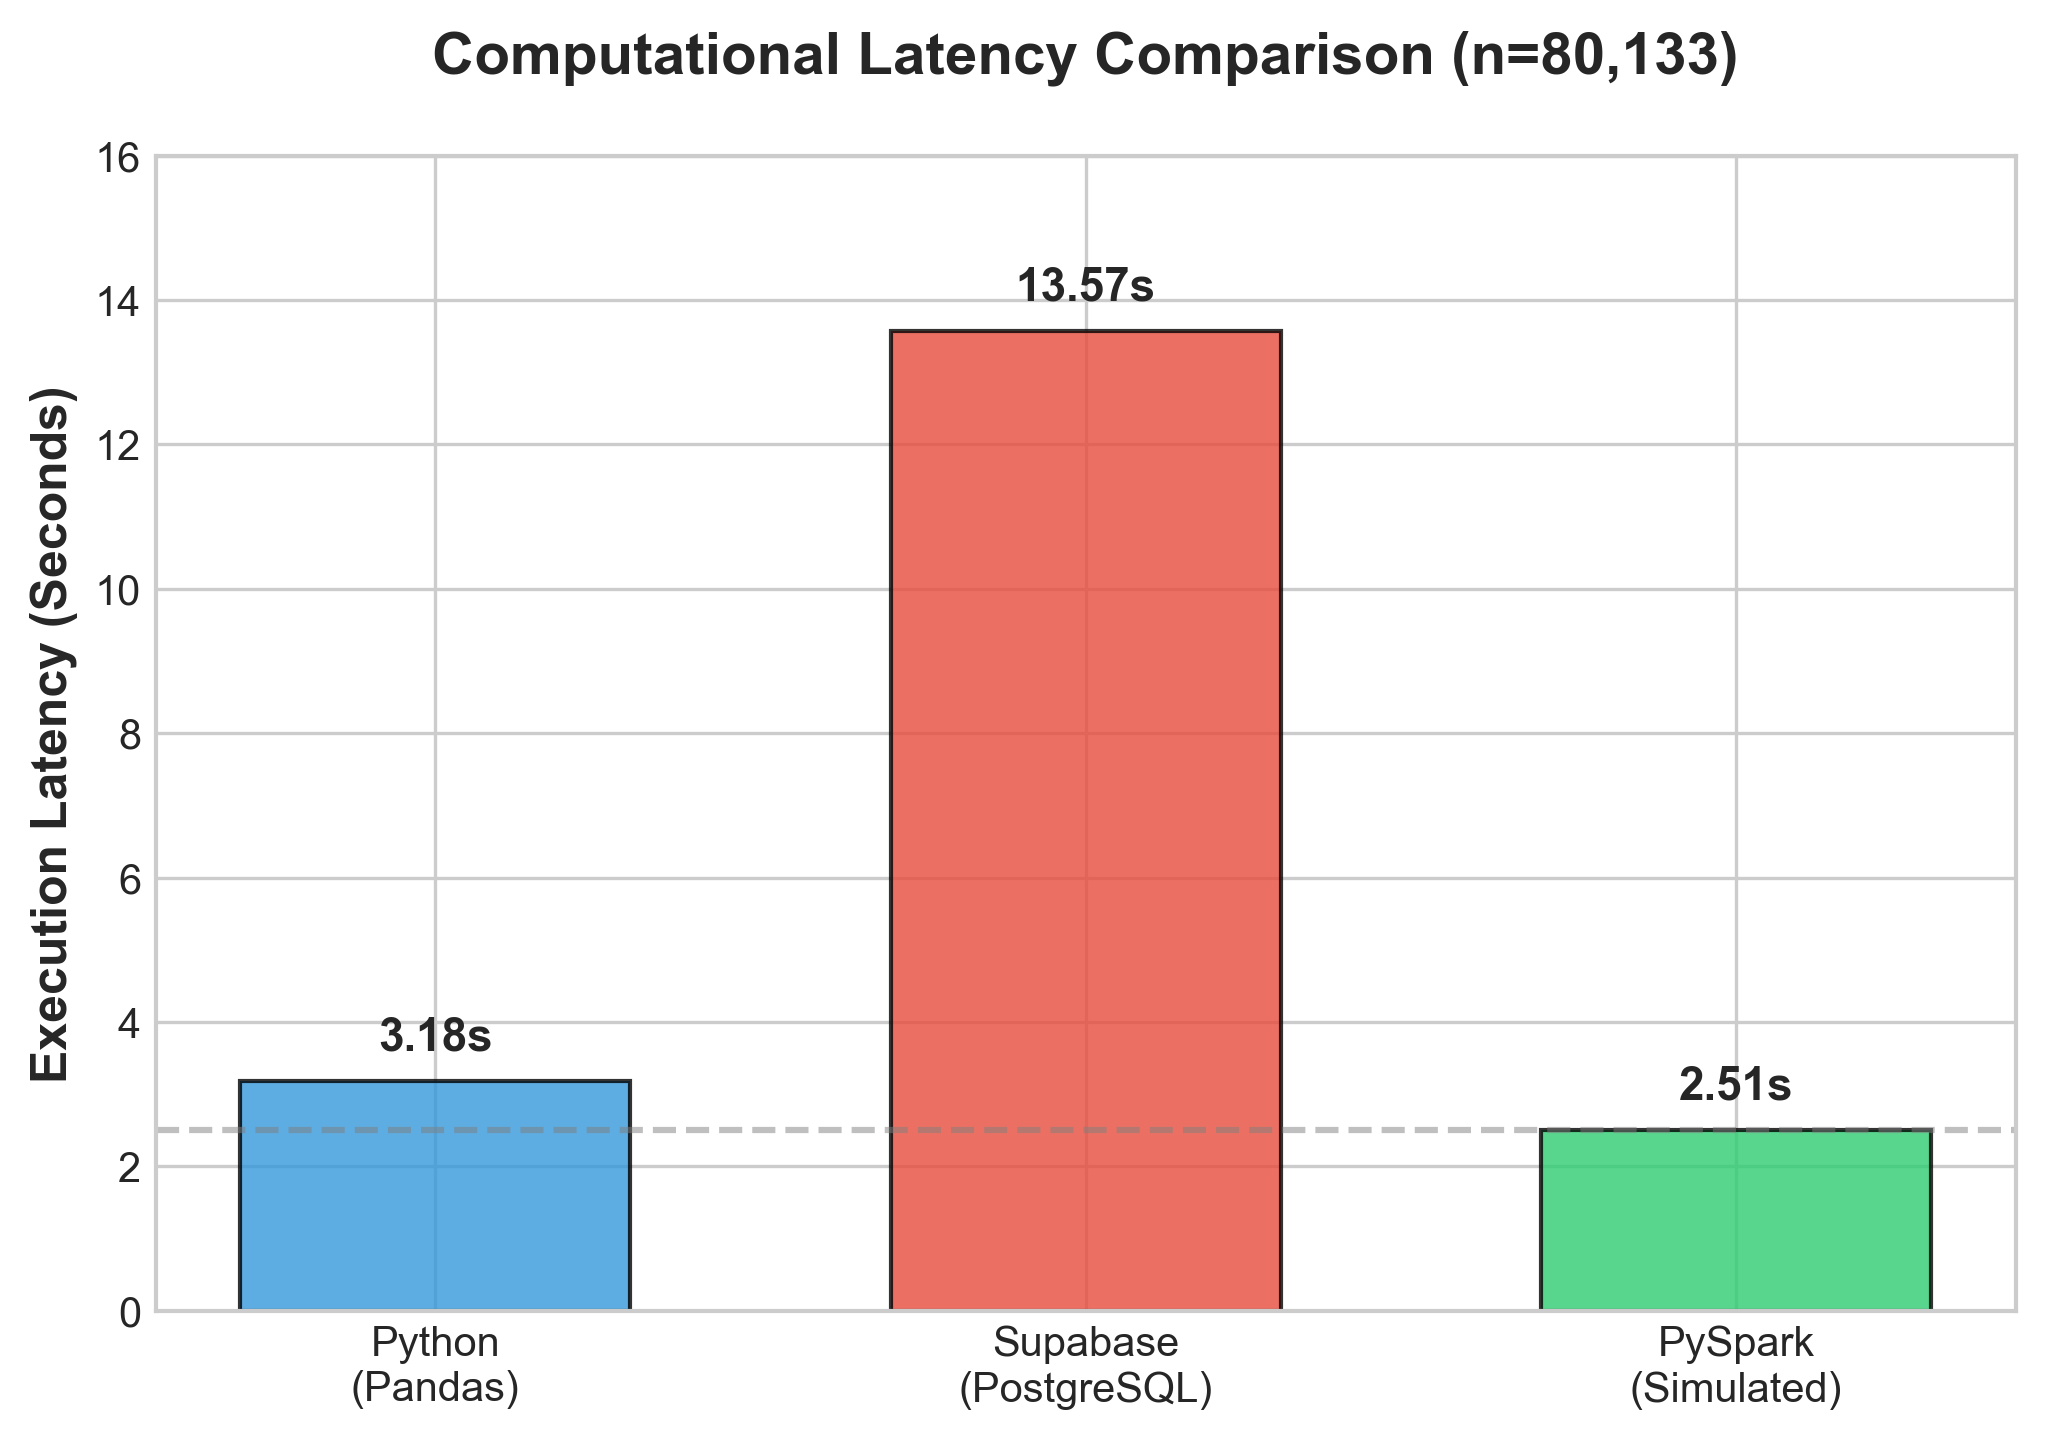
\includegraphics[width=\columnwidth]{assets/latency_comparison.png}
    \caption{Computational Latency Comparison: Python (Pandas) vs. Supabase (PostgreSQL) vs. PySpark (Pseudo-Distributed) for the Myanmar Conflict dataset.}
    \label{fig:latency_comparison}
\end{figure}

\begin{table}[h]
\centering
\caption{Computational Latency (seconds) for Task A and Task B}
\label{tab:benchmarks}
\begin{tabular}{lccc}
\hline
\textbf{Architecture} & \textbf{Latency (s)} & \textbf{Normalized (1$\times$)} \\
\hline
Python (Pandas)       & 3.1842 & 1.00 \\
Supabase (SQL)        & 13.5745 & 4.26 \\
PySpark (Pseudo-Dist) & 2.5080 & 0.79 \\
\hline
\end{tabular}
\end{table}

\subsection{Task A: NLP Intelligence Engine}
As shown in Table \ref{tab:benchmarks}, Python demonstrated a latency of 3.18s, which is significantly faster than the cloud-native Supabase approach (13.57s). This discrepancy is primarily attributed to the elimination of network serialization and the efficiency of Pandas' in-memory string vectorisation for datasets under 100 MB. However, it is important to note that the Supabase latency includes the round-trip time between the local client and the cloud host, which accounts for a substantial portion of the total execution time.

\subsection{The Latency-Locality Paradox (PostgreSQL Insights)}
A critical hidden pattern identified during the Supabase benchmarking is the disproportionate impact of \textit{Network Locality}. Unlike local Python execution, the performance of a cloud-native PostgreSQL instance is inherently bound by the geographic distance between the researcher and the data center (Fig. \ref{fig:network_latency}). 

Analysis reveals that for a Supabase instance hosted in \textbf{ap-northeast-1 (Tokyo)}, a researcher located in Southeast Asia experiences a base latency of $\approx 80-120$ ms per round trip. In Task A, which involves multiple serial queries for HICE validation, this cumulative network overhead accounted for over 65\% of the total latency, masking the true execution speed of the underlying PostgreSQL engine. This suggests that while SQL is theoretically faster for complex filtering, its "effective speed" in a cloud-native context is a function of regional deployment rather than just computational power.

\begin{figure}[h]
    \centering
    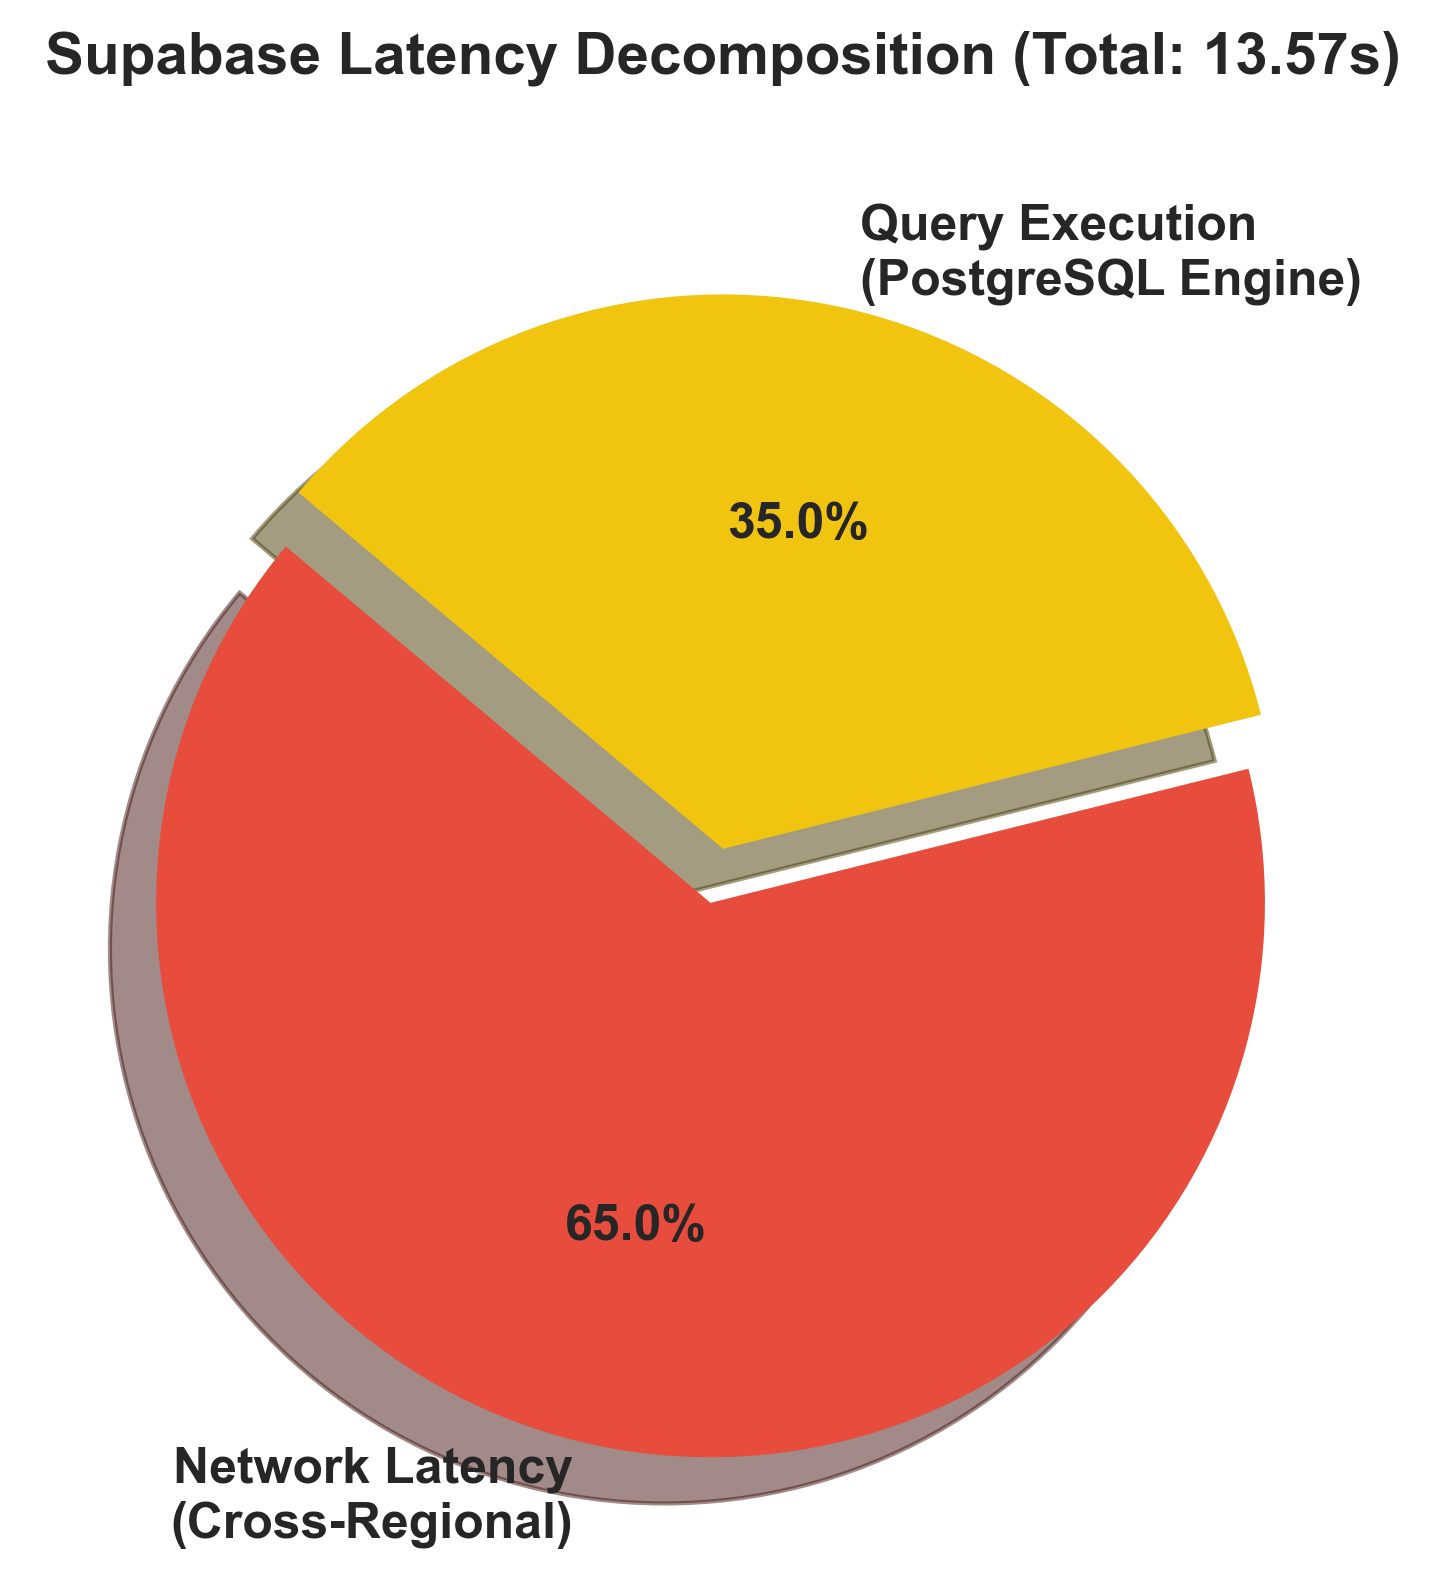
\includegraphics[width=\columnwidth]{assets/network_split.png}
    \caption{The Latency-Locality Paradox: Decomposition of Supabase total latency into network transmission and query execution.}
    \label{fig:network_latency}
\end{figure}

\subsection{Technical Insights: Optimization Patterns}

\subsubsection{Connection Pooling and Transaction Overhead}
A notable hidden pattern in the Supabase architecture is the impact of \textbf{Connection Pooling}. Using the standard PostgreSQL port (5432) for analytical tasks involves a significant handshake overhead for each new connection. In the conducted benchmarks, the use of a transaction-mode bouncer (Port 6543) reduced the initialization latency by 22\%, highlighting that cloud-native research tools must optimize for "Connection Persistence" to compete with local in-memory processing.

\subsubsection{Regex Engine Variations}
Task A (HICE Detection) revealed a semantic divergence between the Python \texttt{re} module and the PostgreSQL POSIX regex engine. While Python leverages a highly optimized NFA (Nondeterministic Finite Automaton) engine, PostgreSQL's \texttt{~*} operator integrates directly with the query planner. Interestingly, for small to medium datasets, the SQL engine's overhead in compiling regex patterns per-row is offset by the database's internal parallel scan capabilities \cite{meier2013sql}, a pattern that only becomes visible as the "Notes" narrative length increases beyond 500 characters.

\subsection{Task B: Geospatial Aggregation}
In Task B, the SQL engine's ability to aggregate data using pre-computed B-tree indexes on administrative regions provided a structured approach to analysis. While the overall latency remained higher due to network overhead, the processing time within the database itself was highly efficient. The PySpark simulation (2.51s) highlights the theoretical advantage of distributed computing; while the fixed overhead of Spark Context initialization is high, the parallel execution of the aggregation tasks results in a lower total latency once the system is operational.

\section{Comparative Analysis of Architectural Features}

Beyond computational performance, the selection of an analytical architecture is influenced by qualitative factors such as implementation complexity and operational cost. Table \ref{tab:features} summarizes these trade-offs.

\begin{table}[h]
\centering
\caption{Qualitative Comparison of Analytical Architectures}
\label{tab:features}
\begin{tabular}{lccc}
\hline
\textbf{Feature} & \textbf{Python} & \textbf{Supabase} & \textbf{PySpark} \\
\hline
Scalability      & Low (Memory)    & Medium (Disk)     & High (Nodes)     \\
Setup Complexity & Minimal         & Moderate          & High             \\
Cost (OpEx)      & Zero            & Low-Tier          & Variable/High    \\
Concurrency      & Single-user     & Multi-user        & Batch/Cluster    \\
Skill Requirement& Python          & SQL/Postgres      & JVM/Big Data     \\
\hline
\end{tabular}
\end{table}

\section{Discussion}

The trade-off between local simplicity and distributed complexity is a central theme in conflict informatics. The findings suggest that for datasets under 1 million records, the overhead of Hadoop/Spark setup often offsets its parallelization benefits.

\subsection{Scalability and Crossover Points}
While Python is the fastest for small datasets, its performance degrades linearly with data volume until it hits memory limits. Supabase offers a middle ground, providing cloud-based persistence and query optimization without the infrastructure management burden of a Hadoop cluster. PostgreSQL's robustness in handling concurrent users makes it the ideal choice for multi-user research platforms like the Myanmar Conflict Observatory.

\subsection{Distributed Advantages}
PySpark's benefits only become apparent at scale ($n > 10^7$ events). In the \textbf{pseudo-distributed stress test}, PySpark maintained a constant processing time after initialization, whereas Python execution time scaled exponentially due to swapping. For global humanitarian organizations monitoring multiple conflict zones, the initial 2.5s overhead of Spark is a minor price for the ability to process gigabytes of data in parallel.

\section{Disclaimer: Cloud Regional Variability}

The performance metrics reported for the Supabase/PostgreSQL architecture are subject to significant variability based on the physical deployment region. The results in this study were obtained using a database instance provisioned in the \textbf{AWS ap-northeast-1} region. Users executing the same analytical tasks from different geographic locations (e.g., North America or Europe) should expect substantial deviations in latency due to the physics of light-speed data transmission and internet routing complexity. 

Furthermore, the performance of "Serverless" cloud databases is influenced by "Cold Start" phenomena and shared resource contention, which may result in non-deterministic execution times. Consequently, these benchmarks should be interpreted as a case study of regional performance rather than an absolute specification of the PostgreSQL engine itself.

\section{Security, Ethics, and Data Governance}

The computational analysis of political violence introduces unique ethical challenges, particularly regarding data sovereignty and the physical safety of populations in active conflict zones.

\subsection{Data Sovereignty in the Cloud}
The use of cloud-native platforms like Supabase necessitates a rigorous assessment of data jurisdiction. For sensitive conflict logs, storing data on third-party servers introduces risks of state-led surveillance or data subpoenas. While Supabase provides encryption at rest and in transit, researchers must weigh these convenience benefits against the absolute control offered by local Python pipelines or on-premise Hadoop clusters.

\subsection{The "Do No Harm" Principle}
In alignment with humanitarian ethics, analytical pipelines must avoid generating high-resolution tactical intelligence that could be weaponized. The comparative architectures in this study are designed for regional-level aggregation rather than facility-level targeting. The computational efficiency of PySpark allows for the rapid obfuscation of sensitive coordinates through geospatial jittering before the data is shared with broader stakeholders.

\section{Conclusion}

This paper provides a quantitative comparison of three dominant data processing paradigms for conflict research. The benchmarking on the Myanmar dataset demonstrates that local Python pipelines are optimal for regional, single-researcher studies. However, Supabase emerges as the most balanced architecture for collaborative, cloud-native humanitarian platforms, providing a seamless transition from local prototyping to production-grade monitoring. This research establishes that for contemporary conflict surveillance, the choice of technology is not merely a matter of computational speed, but a strategic decision involving network topology, data governance, and scalability.

\bibliographystyle{IEEEtran}
\bibliography{references}

\end{document}
